 % -*- encoding: UTF8 -*-
%
%%
%%*****************************************************************************
%%
%%
\chapter{Conclusion \& Outlook}

%The main goal of this work was the realization of a novel single-fiber-based scanning scheme enabling simultaneous 3D OCT in combination with full field microscopy using spectrally separated beampaths in a probe with dimensions of only $13 \times 2 \times \SI{3}{\milli\meter^3}$. 

The main goal of this work is the realization of a novel fiber scanner for 3D OCT imaging, designed for its combination with a full field microscope to form a multimodal probe. A tubular piezoelectric fiber scanner is used to perform en face scanning required for 3D OCT measurements. The complete scanning engine has an outer diameter of \SI{0.9}{\milli\meter} and a length of \SI{9}{\milli\meter}, and features custom fabricated \SI{10}{\micro\meter} thick polyimide flexible interconnect lines to address the four piezoelectric electrodes. This scanning engine was tested in a single modality, demonstrator probe with an external diameter of \SI{2.5}{\milli\meter} and a total length of \SI{15}{\milli\meter}, allowing the OCT imaging of a \SI{1}{\milli\meter} field of view with a resolution of \SI{45}{\micro\meter} using \SI{1330}{\nano\meter} light. 

To the best of our knowledge, the presented demonstrator probe is also one of the most compact implementation of an OCT microendoscope.

\section{Conclusion}
During this project, the behavior of fiber scanners was analyzed and several approaches were discussed and simulated. It was concluded that its implementation as fourier plane scanner using a GRIN lens as collimator and weight was optimal for OCT. A complete electro-mechano-optical analysis and simulation followed, allowing the optimization of the system to reach diffraction-limited resolution and a maximum field of view.

The size constraints that required the implementation of the scanner in a $1\times \SI{1}{\milli\meter^2}$ channel in the bottom of the bench challenged the electrical contacting of the \SI{800}{\micro\meter} diameter piezoelectric actuator. The solution involved the fabrication of a novel \SI{10}{\micro\meter} thick polyimide ribbon cable that can be rolled around the tube and contacted to it using vias and conductive glue. The cleanroom process proved to be reliable and repeatable, encouraging its use in upcoming projects.

This work also demonstrated the bonding of a single mode, \SI{80}{\micro\meter} optical fiber to a GRIN lens using a custom silicon microfabricated tool. This method allowed a placement accuracy in the \SI{}{\micro\meter} range, creating an optical and mechanical bond that operates reliably under the high mechanical stress found in a resonant scanner. Prior OCT setups including GRIN lenses showed that they can cause problematic backreflections. This problem was successfully avoided by a custom GRIN lens design with a \SI{1}{\degree} tilted exit facet. This solution, together with an special attention to the layout of the optical components, resulted in an optical system with backreflections below 0.02\%.

The assembly of the single mode demonstrator was successfully achieved using alignment features integrated in a 3D-printed housing. This part was manufactured using a commercial, low cost stereolithographic resin printer that enabled quick iterations of the design. The manufactured demonstrator allowed the analysis and proof of concept of the fiber scanner concept. Experimental measurements helped refining the assumptions used in the analytical calculation of the resolution of OCT systems. The resultant theoretical description, which closely matches experimental results, will help in the design of future OCT and confocal systems. Although previous work at IMTEK had proven the use of fiber scanners for confocal imaging \cite{Meinert}, further analysis was needed to understand and correct for the imaging distortions caused by whirling. The calibration method used in this work, which can operate in real time, reduces the imaging distortions to a minimum and enables the quantitative analysis of the acquired image. This enabled going one step further in cooperation with the Medical University Vienna, where the OCT imaging concept was proven, creating new opportunities for collaboration. 

\section{Outlook}
This thesis sucessfully achieved OCT imaging within the demonstrator probe. Thus, the next step is to integrate the scanner in the bimodal probe, as described in \cite{vilches}. A render of the proposed bimodal probe is shown in \autoref{fig:bimodalRender}. As the optical system of the demonstrator is designed to emulate that of the bimodal probe, the same optical performance is to be expected. 

\begin{figure}[h!]\centering
      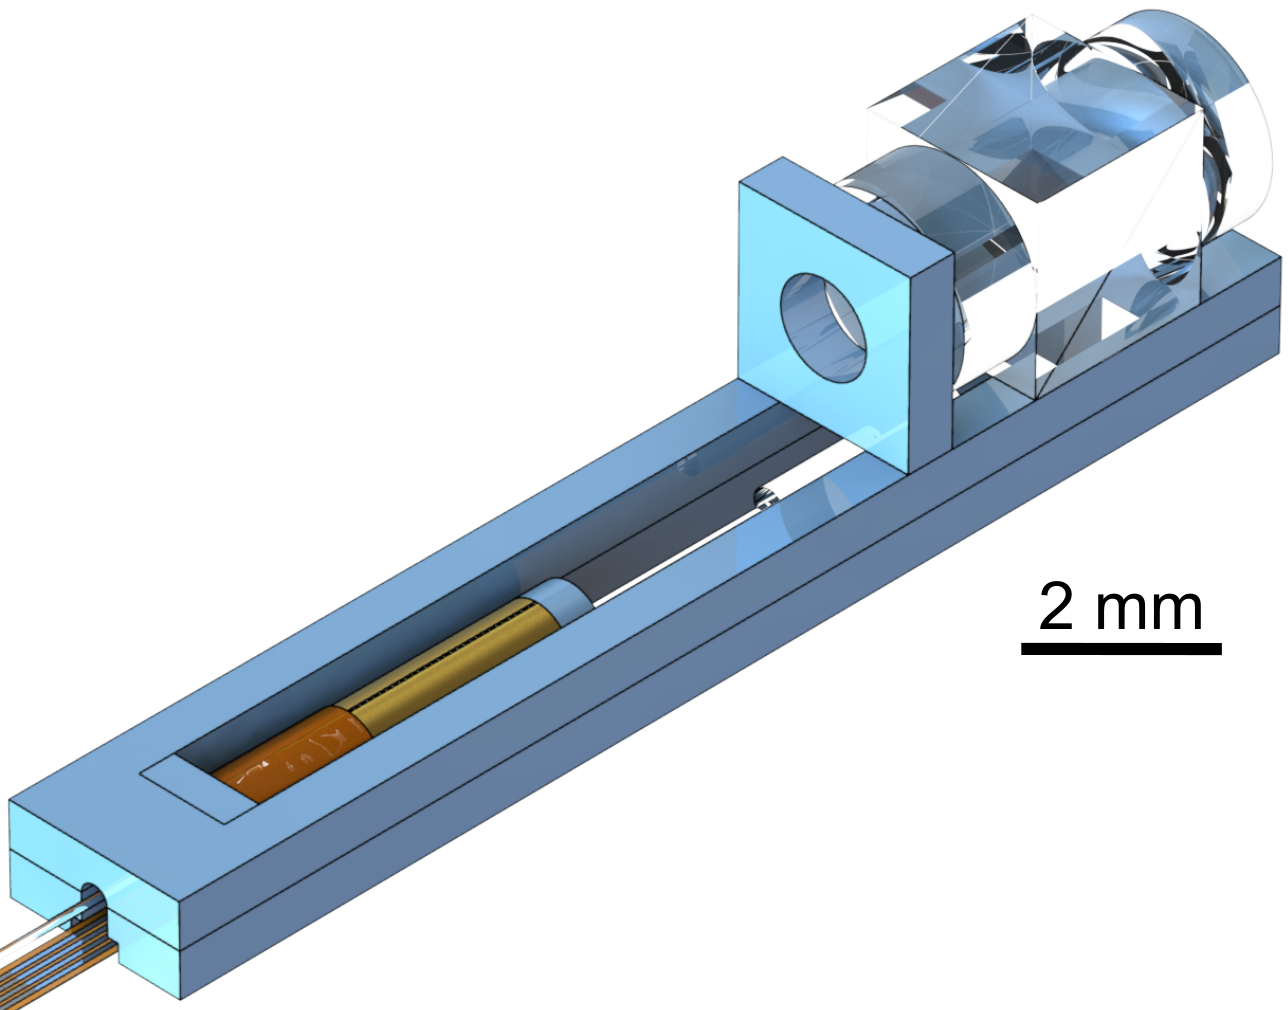
\includegraphics[width = 8cm]{figures/60_Conclusion/bimodalRender.png}
      \caption{CAD image of the proposed bimodal probe, integrating the fiber scanner in the silicon bench. \cite{vilches} }
      \label{fig:bimodalRender}
\end{figure}
